\chapter{Iterative design} \label{iterative}
% \section{Motivation for a Complementary Optimization Strategy}
The fundamental problem in the examples 
    in chapters \ref{direct} and \ref{regularized}
    is actually not in the methods themselves, 
    but in the improper selection of a target field. 
In fact, it is very difficult to select a suitable target field 
    because not every field even has a manufacturable dielectric structure 
    that is able to reproduce it. 
Furthermore, it is nearly impossible to select a multi-dimensional field 
    which corresponds to a well-behaved, isotropic and 
    discretely-valued $\epsilon$, 
    as would be needed for practical structures. 

What we realized was that a successful method 
    must be allowed to modify the target field as well as 
    its dielectric structure.
This realization led us to an iterative design strategy for nanophotonic devices.

\section{Problem formulation}
We start with the same target field as in the previous examples 
    but we now allow for it to be modified during the design process. 
Specifically, we alternate between modifying $z$ (structure) 
    to better fit $x$ (field), 
    and then modifying the $x$ (field) to better fit $z$ (structure):
    \begin{subequations}\begin{align} 
    \minimize_z & \|A(z)x - b\|^2 + \eta_0\|z - z_\text{prev}\|^2 \\
    \minimize_x & \|A(z)x - b\|^2 + \eta_1\|x - x_\text{prev}\|^2,
    \end{align}\end{subequations}
which can be more succintly expressed as 
    \BE \minimize_\text{alternately $x$ then $z$} 
        \|A(z)x - b\|^2 + \eta_0\|z - z_\text{prev}\|^2
                        + \eta_1\|x-x_\text{prev}\|^2. \label{iterative problem}\EE

In this formulation, both structure ($z$) and field ($x$) variables
    have regularization terms.
In order to avoid the performance/manufacturability trade-off 
    encountered in chapter~\ref{regularized},
    we decrease the values of $\eta_0$ and $\eta_1$ at each subsequent iteration.

\section{Implementation}
The most notable implementation difference is that,
    in contrast to direct design,
    \eq{iterative problem} must be solved multiple times
    in order to arrive at a good design.
Thus, design times now increase from seconds to minutes.

Note that, in order to design two-dimensional structures,
    \eq{iterative problem} is only modified in the
    definition of its constituent vectors and matrices,
    the formulation remains the same.


\section{Results}
\subsection{1D}
Fig.~\ref{comp pic} shows that the iterative algorithm, after $400$ iterations and with the correct choice of regularization parameters $\eta_0$ and $\eta_1$, results in a well-behaved structure that is able to closely reproduce the modified target field\cite{Lu10}. 

\begin{figure}[htbp]\centering
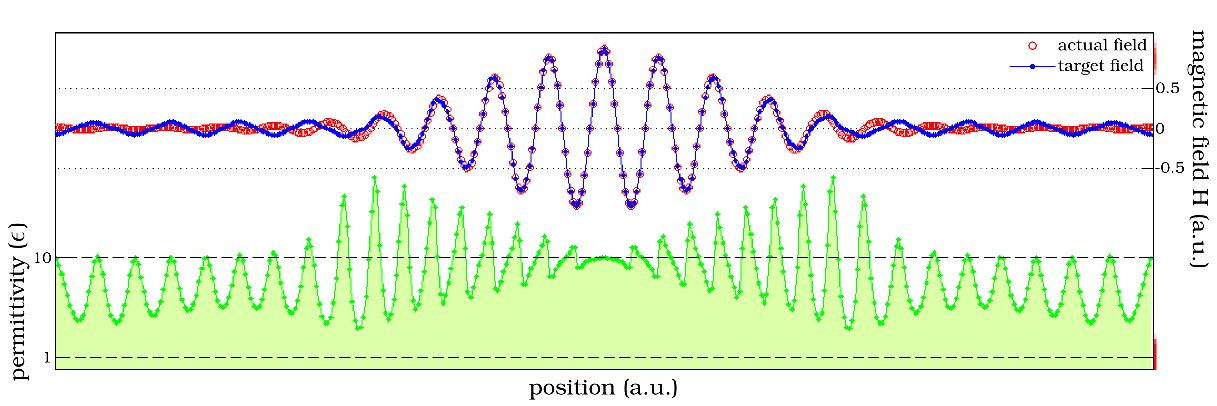
\includegraphics[width=\textwidth]{p1/complementary}
\caption{Iterative design of a one-dimensional resonator. 
    The target field in Figs \ref{p1:direct} and \ref{regls pic} is used as the initial target field. The rates of change for both $\epsilon$ and $H$ are controlled by regularization parameters $\eta_0=10^{-4}$ and $\eta_1=10^{-3}$ respectively. The $400$ iterations used to achieve this result took $60$ seconds to compute. This method results in a well-behaved $\epsilon$ that actually produces a field very similar to the original target field. Interestingly, the formation of a ``steady-state'' periodic structure toward the sides of the structure has emerged.}
\label{comp pic}
\end{figure}

\subsection{2D}
The iterative design method can also be extended to two dimensions\cite{Lu10}.
We demonstrate this using an S-shaped target field 
    which is non-trivial to reproduce. 
The design result is shown in fig.~\ref{S pic}. 
    The resulting dielectric structure is continuous, unbounded and 
    contains very few singularities (white dots), 
    but the final target and actual fields match up well. 
Also, the computational cost remains quite reasonable; the $50$ iterations needed required only $5$ minutes of computation time. 
\begin{figure}\centering
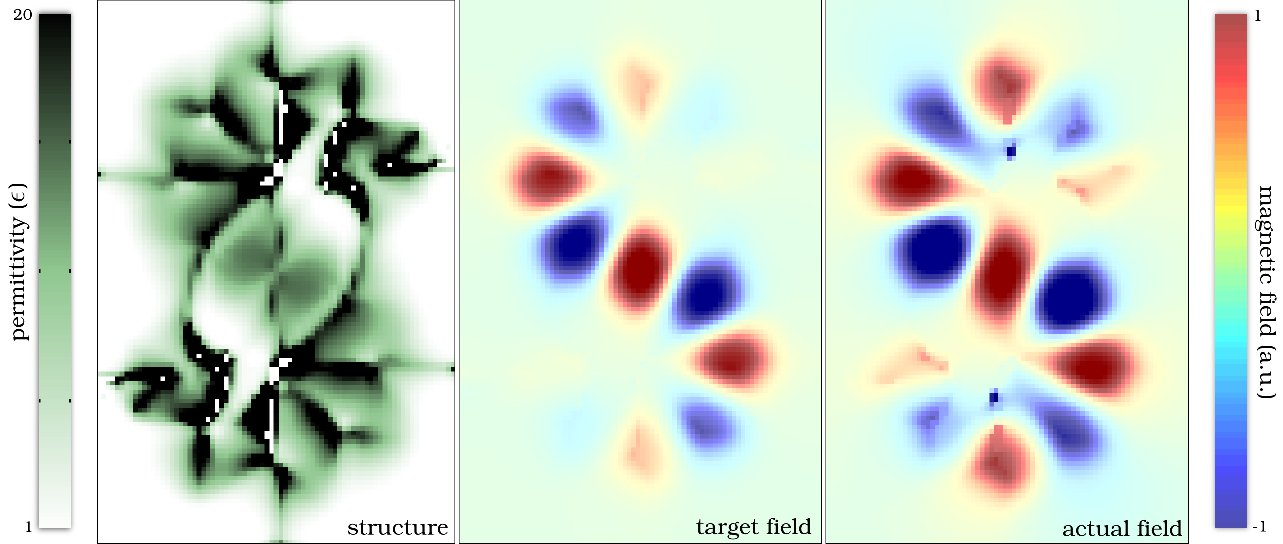
\includegraphics[width=\textwidth]{p1/S}
\caption{Iterative design of an ``S'' resonator. 
The design was initialized by specifying an initial dielectric structure ($\epsilon=1$ everywhere) and a resonant field in the shape of an ``S''. 
The final dielectric structure was produced after $50$ iterations which took $90$ seconds to complete in total. The grid size was $80\times 120$. The final dielectric structure is quite unintuive, and yet reproduces the target field surprisingly well. This example demonstrates the versatility of the iterative design method in producing designs, from very simple specifications, which otherwise could be attained only with considerable difficulty.}
\label{S pic}
\end{figure}

\chapter{Iterative design with bounded $\epsilon$} \label{bounded}
\section{Problem formulation}
In order to achieve a more practical, discretely-valued dielectric structure, we can impose strict upper- and lower-bounds on the structure ($z$). 
To this end, we can modify \eq{iterative problem} as such,
    \begin{subequations}
    \begin{align} 
    \minimize & \|A(z)x - b\|^2 + \eta_1\|x - x_\text{prev}\|^2\\
    \subto & z_\text{min} \le z \le z_\text{max}. 
    \end{align}\label{bounded problem}
    \end{subequations}
Here, the regularization term for $z$ has been replaced by hard constraints
    on the values that $z$ can take on.

This modification takes us one step closer to producing manufacturable structures,
    which must be discretely valued.

\section{Implementation} 
In this algorithm, \eq{bounded problem} is no longer linear in $z$
    but is still convex\cite{Boyd04}.
For this reason, the \emph{CVX} package\cite{Grant09}, 
    a Matlab-based modeling system for convex optimization, 
    is now used to solve \eq{bounded problem} for $z$.

\section{Results}
\subsection{1D}
Once again, we attempt the design of a one-dimensional resonator
    and find that a nearly binary-valued dielectric structure is obtained,
    as seen in fig.~\ref{bounded comp pic}\cite{Lu10}.
Note that the the directly discreteness of $z$ was not enforced (since that would make the problem non-convex); 
    however, a discrete, binary-valued structure arose fortuitously. 
Critically, this dielectric structure accurately produces the final target field. 

\begin{figure}[htbp]\centering
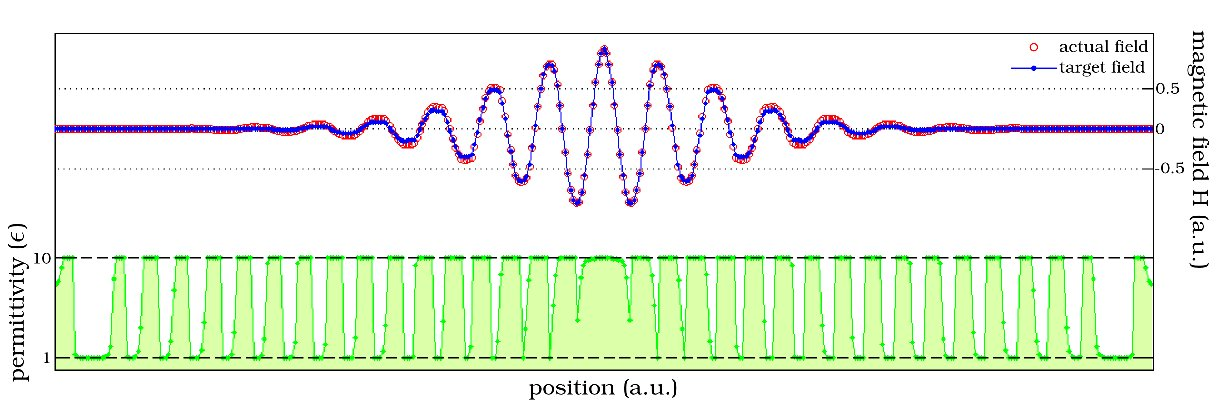
\includegraphics[width=\textwidth]{p1/bounded}
\caption{Iterative design of a one-dimensional structure with bounded $\epsilon$. 
    The parameters are identical to those used to produce Fig.~\ref{comp pic} with the exception that only one regularization term is now needed ($\eta_2=10^{-3}$). The algorithm was run for $100$ iterations, which took $100$ seconds. The structure turns out to be almost completely binary-valued and looks like a periodic structure with tapered duty cycle. It produces an actual field which very closely matches the final target field.}
\label{bounded comp pic}
\end{figure}

\subsection{2D}

We now use the complementary optimization method to design resonators with discrete, binary $\epsilon$ in two dimensions\cite{Lu10}.

Fig.~\ref{circle pic} shows the design of a circular grating resonator. 
The dielectric structure emerged from a very simple choice of initial structure, 
    namely a constant $\epsilon=12.25$ everywhere. 
The range of $\epsilon$ was limited to be from $1$ to $12.25$.
Additionally, the components of $\epsilon$ outside a specified circle 
    were held at a constant $\epsilon=12.25$ 
    for the duration of the design process. 
The entire algorithm was run for $40$ iterations and took $7$ minutes.
Interestingly, the central bowtie-like structure has emerged 
    from previous genetic optimization methods as well\cite{Gond08}. 

\begin{figure}[htbp]\centering
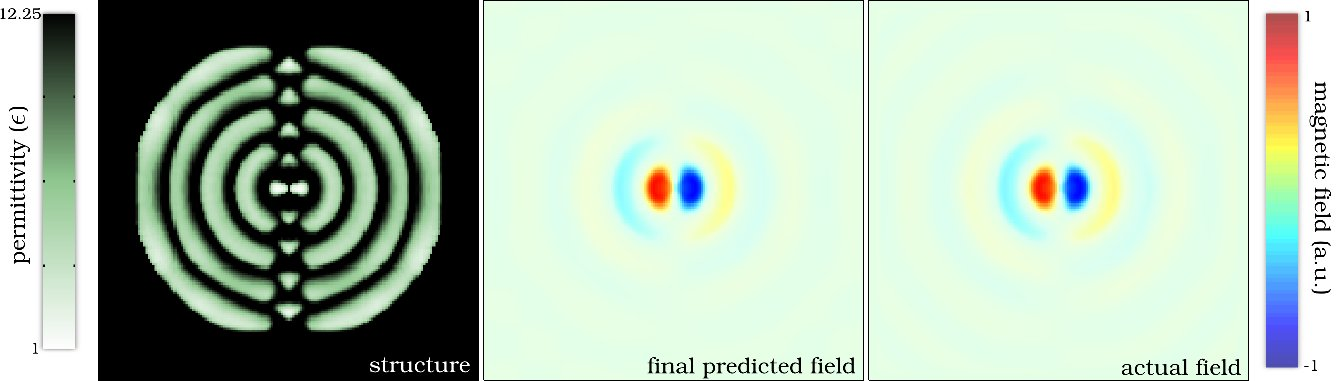
\includegraphics[width=\textwidth]{p1/circle}
\caption{Iterative design of a two-dimensional resonator 
            with hard constraints on $\epsilon$.
    The values of $\epsilon$ are only allowed to be modified within a central circular region and must be kept between $1$ and $12.25$. 
    After $40$ iterations on a $160 \times 160$ grid, which took $7$ minutes to complete, a discrete structure emerged with excellent match between the predicted ($x_{40}$) and actual fields. 
    The structure resembles a circular grating with a bowtie-like central structure for focusing the resonant energy to a single point.} 
\label{circle pic}
\end{figure}

The same approach was used to design a beam resonator 
    as shown in Fig.~\ref{line pic}. 
The parameters used in this design are identical 
    to those used for the circular resonator, 
    with the exception that the initial dielectric structure 
    now consists of an unbroken waveguide, 
    and the region where $\epsilon$ can be modified is now confined 
    to the center of the waveguide.

\begin{figure}[htbp]\centering
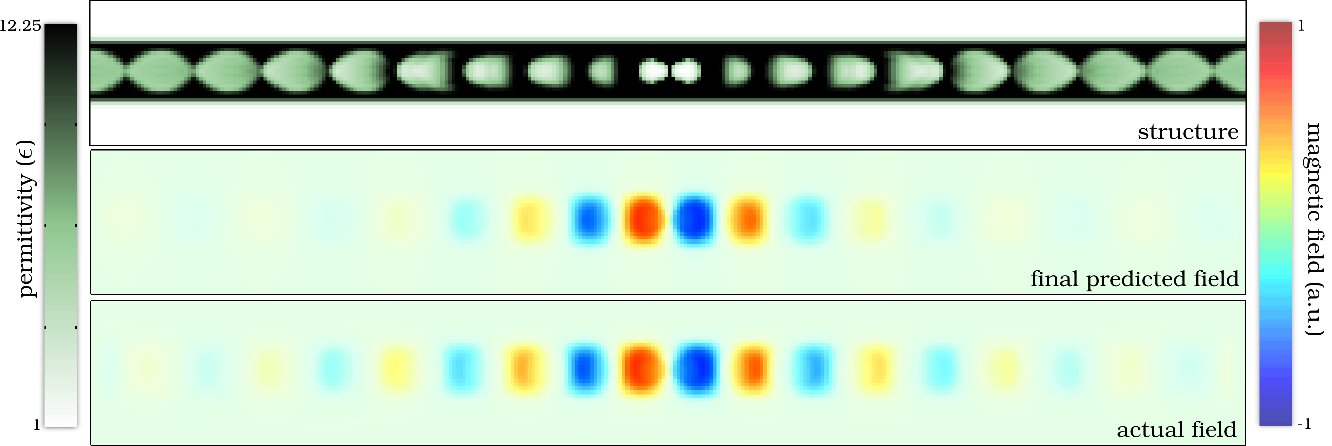
\includegraphics[width=\textwidth]{p1/beam}
\caption{Iterative design of a beam resonator in two dimensions 
        with bounded $\epsilon$. 
    The initial conditions are identical to those for Fig.~\ref{circle pic}, 
        except that the initial dielectric structure is an unbroken waveguide, 
        and $\epsilon$ can only be modified within that waveguide. 
    The structure emerged after $40$ iterations on a $320\times 40$ grid, 
        which took $5$ minutes of computation. 
    The bowtie-like structure has reappeared in the center.}
\label{line pic}
\end{figure}






% 
% \documentclass[10pt,letterpaper]{article}
% \usepackage{opex3}
% \usepackage{amsmath}
% \usepackage{graphicx}
% 
% \begin{document}
% \title{Inverse design of a three-dimensional nanophotonic resonator}
% \author{Jesse Lu, Stephen Boyd, and Jelena Vu\v{c}kovi\'{c}}
% \address{Stanford University, \\ Stanford, C.A., 94305}
% \email{jesselu@stanford.edu}
% 
% 
% \begin{abstract} 
% The inverse design of a three-dimensional nanophotonic resonator is presented. The design methodology is computationally fast (10 minutes on a standard desktop workstation) and utilizes a 2.5-dimensional approximation of the full three-dimensional structure. As an example, we employ the proposed method to design a resonator which exhibits a mode volume of $0.32(\lambda/n)^3$ and a quality factor of $7063$. % 8808 35648
% \end{abstract}
% 
% \ocis{(230.5750) Resonators.} % REPLACE WITH CORRECT OCIS CODES FOR YOUR ARTICLE
% 
% %%%%%%%%%%%%%%%%%%%%%%% References %%%%%%%%%%%%%%%%%%%%%%%%%
% \begin{thebibliography}{99}
% \bibitem{miller} D. A. B. Miller, ``Rationale and challenges for optical interconnects to electronic chips,'' Proc. of the IEEE \textbf{88}, 728-749 (2000).
% \bibitem{prevwork} J. Lu and J. Vuckovic, ``Inverse design of nanophotonic structures using complementary convex optimization,'' Opt. Express \textbf{18}, 3793-3804 (2010).
% \bibitem{inan} U. Inan, A. Inan, \emph{Electromagnetic Waves} (Prentice Hall, 2000), page 296.
% \bibitem{yee} K. Yee, ``Numerical solution of initial boundary value problems involving maxwell's equations in isotropic media,'' IEEE Trans. Antennas Propag. Mag. \textbf{14}, 302-307 (1966).
% \bibitem{boydbook} S. Boyd and L. Vandenberghe, \emph{Convex Optimization} (Cambridge University Press, 2004).
% \bibitem{altdir} S. Boyd, N. Parikh, E. Chu, B. Peleato, and J. Eckstein are preparing a manuscript to be called, ``Distributed Optimization and Statistical Learning via the Alternating Direction Method of Multipliers,'' \verb+http://www.stanford.edu/~boyd/papers/distr_opt_stat_learning_admm.html+. 
% \bibitem{cholmod} Y. Chen, T. A. Davis, W. W. Hager, and S. Rajamanickam, ``Algorithm 887: CHOLMOD, supernodal sparse Cholesky factorization and update/downdate,'' ACM Trans. Math. Software \textbf{35}, No. 3, 2009.
% \bibitem{cvx} M. Grant and S. Boyd, \emph{CVX: Matlab software for disciplined convex programming}, version 1.21. \verb+http://cvxr.com/cvx+, January 2011.
% \bibitem{digitize} D. Englund, I. Fushman, and J. Vuckovic, ``General recipe for designing photonic crystal cavities,'' Opt. Express \textbf{13}, 5961-5975 (2005).
% \end{thebibliography}
%  
% %%%%%%%%%%%%%%%%%%%%%%%%%%  body  %%%%%%%%%%%%%%%%%%%%%%%%%%
% \section{Begin of 2.5 D (Motivation)}
% To date, the design of nanophotonic devices has generally involved a lengthy (days, weeks) process in which one perturbs, by trial-and-error, canonical structures such as photonic crystals or waveguide-coupled rings to achieve the desired performance for the device. 
% 
% Instead, an inverse design method in which the user only specifies the desired electromagnetic field, or characteristics thereof, and then leaves the computer to find a dielectric structure satisfying these requirements, would be a much more intuitive and computationally efficient design strategy. Furthermore, such a method may even be the only feasible option available for the design of more complex multi-wavelength and multi-functional nanophotonic devices needed for on-chip integration\cite{miller}.
% 
\subsection{2.5D}
% \section{2.5-dimensional approximation}
Unfortunately, to directly extend our previous method to full three-dimensional space requires solving for a very large ($\sim 10^7 \times 10^7$) and ill-conditioned matrix, namely that given by the time-harmonic Maxwell's equation in three dimensions, which for the electric ($E$) field is
\begin{align}
\nabla\times\nabla\times E - \mu\omega^2\epsilon E &= 0,\quad\text{where}\label{wave} \\
E &= E(x,y,z).
\end{align}

Therefore, to make our problem more tractable, we formulate a 2.5-dimensional approximation of the electromagnetic fields of a planar three-dimensional nanophotonic device\cite{Lu11}. As shown in Fig.~\ref{approx}a, this involves treating a planar three-dimensional nanophotonic device as a truncated holey fiber with identical dielectric structure. We take advantage of the planar nature of most nanophotonic devices in this way to produce a tractable, computationally-fast method. The $E$-field inside such a holey fiber is expressed as
\begin{equation}
E = E(x,y)e^{-i\beta z},
\end{equation}
where $\beta$ is the wave-vector along the fiber axis. Solving for Eq.~\ref{wave} now requires solving for a much smaller ($\sim 10^5 \times 10^5$) matrix, which can be accomplished using standard linear algebra packages. This simulation technique is thus very similar to a two-dimensional finite-difference frequency-domain solver.

As an example, in Fig.~\ref{approx}b, we compare the 2.5-dimensional electric field against the three-dimensional simulated electric field (at the central plane of the slab), given by a standard finite-difference time-domain (FDTD) software package, for an L3 photonic crystal resonator. We see that with the appropriate choice of $\beta$, which we obtain by fitting a sinusoid to the out-of-plane decay in the three-dimensional FDTD solution, our approximation captures most of the characteristics of the three-dimensional field at the center plane of the slab. 
\begin{figure}[hbt]
\centering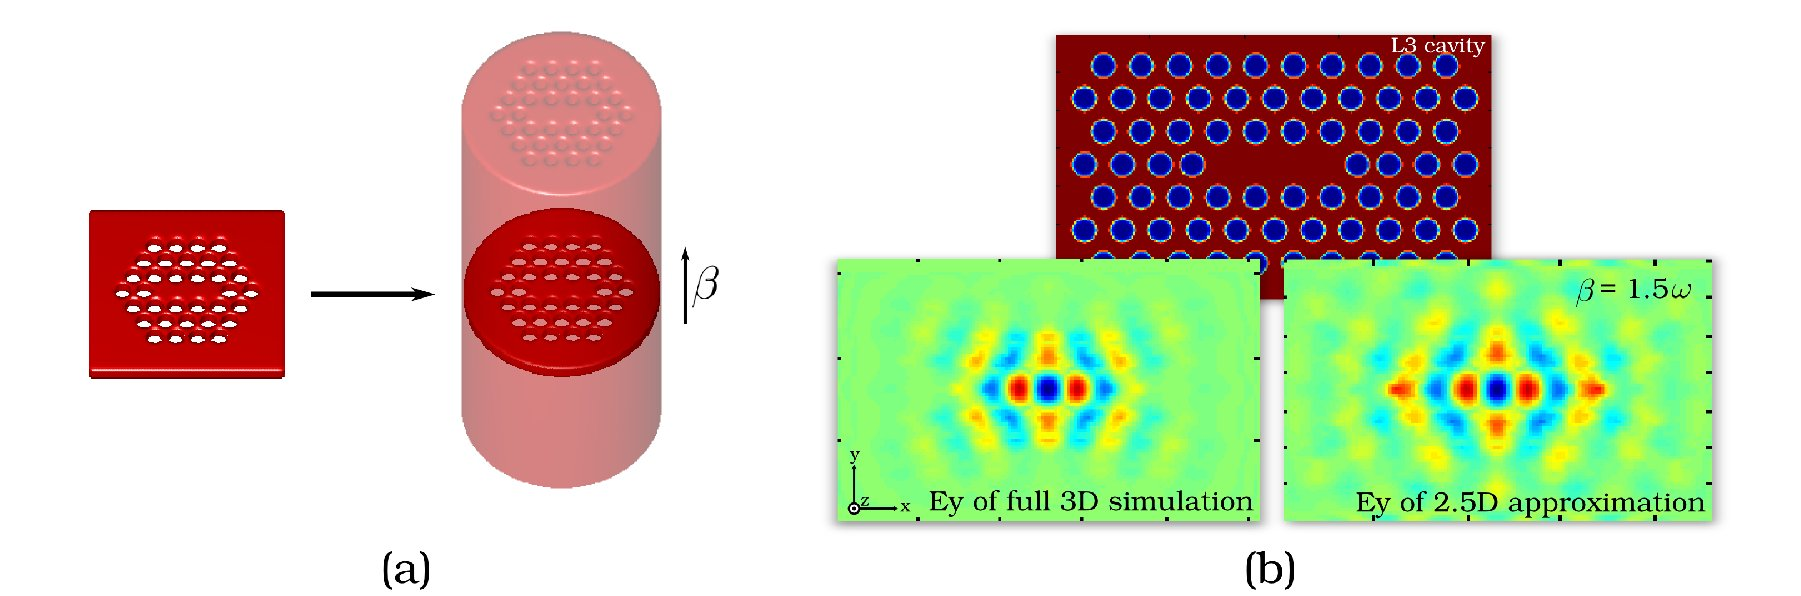
\includegraphics[width=\textwidth]{p2/approx}
\caption{(a) For computational feasibility, the resonant fields of a planar nanophotonic device are approximated as those of a truncated holey fiber with identical dielectric structure. (b) An example of our approximation using an L3 photonic crystal resonator. Most of the characteristics of the full three-dimensional field at the center of the slab appear in the approximate solution.}\label{approx}
\end{figure}

In this approximation, converting from a 2.5-dimensional structure to a full three-dimensional structure only requires the correct choice of slab thickness, $t$, since the in-plane values of $\epsilon$ remain the same. To estimate $t$ for the full three-dimensional device, we treat the resonant mode as a guided mode in a slab waveguide surrounded by a cladding of $n=1$. The expression for $t$ is then the thickness of the slab for the lowest-order TE mode of a slab waveguide with effective refractive index $n_\text{eff}$\cite{Inan00}:
\begin{align}
t &= \frac{2}{\beta}\tan^{-1}\frac{\alpha}{\beta},\label{t} \quad\text{where} \\
\alpha &= \sqrt{k_x^2 - \left(\frac{\omega}{c}\right)^2}, \quad\text{and} \\
k_x &= \sqrt{\left(\frac{n_\text{eff}\omega}{c}\right)^2 - \beta^2}.
\end{align}
Here, $\alpha$ is the wave-vector which determines the evanescent decay of the slab waveguide mode into air, while $k_x$ is an approximated in-plane k-vector. To determine $n_\text{eff}$, the effective refractive index, we use the following approximation,
\begin{equation}
n_\text{eff} = \sqrt{\frac{\|\epsilon E^2\|}{\|E^2\|}}.
\end{equation}
% In the above formulation and for the remainder of the manuscript, the norm ($\|\cdot\|$) refers to the 2-norm over the entire grid and is equivalent to the spatial integral $(\int | \cdot |^2 dr)^{1/2}$.

% 
% In our inverse design method, one proceeds by specifying either the resulting field or its characteristics and then computing a structure which will produce such a field. In this work, we chose to specify the desired field characteristics, namely, small mode-volume and large quality factor. The inverse design problem can then be formulated as,
% \begin{align}
% \text{minimize} \quad& \frac{\|\epsilon E^2\|}{\text{max}\{\epsilon E^2\}} \label{a1}\\ 
% \text{subject to} \quad 
%     & \nabla\times\nabla\times E - \mu\omega^2\epsilon E = 0 \label{a2}\\
%     & \nabla\cdot\epsilon E = 0 \label{adiv}\\
%     & \text{FT}_\text{lightcone}\{E\} = 0, \label{a3} \\
%     & \epsilon = \{\epsilon_\text{air}, \epsilon_\text{silicon}\} \label{a4}
% \end{align}
% where $\epsilon$ and $E$ are the permittivity and electric vector field respectively, defined within the 2.5-dimensional approximation and discretized along a standard Yee grid\cite{yee} with periodic boundary conditions. $\epsilon$ was constrained to be isotropic by only varying $\epsilon_z$ in each cell, and then determining $\epsilon_x$ and $\epsilon_y$ via spatial interpolation. $\text{FT}$ is the two-dimensional Fourier transform.
% 
% In this formulation, the minimization objective (Eq.~\ref{a1}) is the mode volume, which we desire to be as small as possible. Similarily, Eq.~\ref{a3} is a constraint on the electric field to produce a large quality factor by forbidding the existence of any Fourier components within the light cone. Eqs.~\ref{a2} and \ref{adiv} are physical constraints that $\epsilon$ and $E$ must satisfy, that is, the wave equation for the 2.5-dimensional fiber mode and the transversality condition. Lastly, Eq.~\ref{a4} is a binary constraint on epsilon, denoting that we only want the structure to be composed of air or silicon.
% 
% Although our 2.5-dimensional approximation has reduced the size and complexity of the matrices found in the above formulation, the form of the problem in Eq.~\ref{a1}-\ref{a4} is actually incredibly difficult to solve, if for no other reason that Eq.~\ref{a1}, \ref{a2}, and \ref{a4} are non-convex\cite{boydbook} for joint minimization on both $\epsilon$ and $E$. To make matters worse, the binary constraint in Eq.~\ref{a4} generally results in a problem which is NP-hard\cite{boydbook}. For these reasons, our strategy is to employ an alternating directions scheme\cite{altdir}, in which we break Eq.~\ref{a1}-\ref{a4} into two separate, tractable sub-problems which we then solve iteratively.
% 
% \subsection{Alternating directions: field optimization sub-problem}
% The first sub-problem in the alternating directions scheme involves optimizing $E$ while holding $\epsilon$ constant,
% \begin{align}
% \underset{E}{\text{minimize}} \quad& \|\nabla\times\nabla\times E - \mu\omega^2\epsilon E\|
%     + \eta \|\epsilon E^2\| \label{b1}\\ 
% \text{subject to} \quad 
%     & E_\text{center} = 1 \label{bcenter} \\
%     & \nabla\cdot\epsilon E = 0 \label{bdiv}\\
%     & \text{FT}_\text{lightcone}\{E\} = 0, \label{bQ}
% \end{align}
% which is a quadratic problem with linear equality constraints, and is easily solved using a standard factor-solve method for sparse matrices\cite{cholmod}.
% 
% In this sub-problem, the most significant modification to the original formulation in Eq.~\ref{a1}-\ref{a4} is that the constraint in Eq.~\ref{a2} has been relaxed and moved into the minimization objective (Eq.~\ref{b1}). We will denote this term ($\|\nabla\times\nabla\times E - \mu\omega^2\epsilon E\|$) as the \emph{physics residual}. 
% 
% At the same time, the term for the mode volume from Eq.~\ref{a1} has also been modified in Eq.~\ref{b1}. We denote this term ($\|\epsilon E^2\|$) as the \emph{design objective}. Note that although the denominator in the original formulation has been removed in order to make the term convex, the present formulation is still equivalent because we fix the $E$-field in the center of the structure (Eq.~\ref{bcenter}), where we want the maximum to occur. Also note that the constraint in Eq.~\ref{bcenter} is crucial in order to avoid the trivial solution $E=0$.
% 
% Lastly, the $\eta$ coefficient in Eq.~\ref{b1} allows us to trade-off between the physics residual and the design objective. Thus, in order to achieve a small mode volume, the initial value of $\eta$ is large and is subsequently exponentially reduced once per iteration at all points in the grid in order to bring the physics residual to 0. Furthermore, $\eta$ can also be given a spatial weighting in order to reduce in-plane losses; this strategy was implemented in the results presented here.
% 
% 
% \subsection{Alternating directions: structure optimization sub-problem}
% The second sub-problem in the alternating directions scheme involves optimizing $\epsilon$ while holding $E$ constant,
% \begin{align}
% \underset{\epsilon}{\text{minimize}} \quad& \|\nabla\times\nabla\times E - \mu\omega^2\epsilon E\| \label{c1} \\
% \text{subject to} \quad 
%     & \epsilon_\text{air} \le \epsilon \le \epsilon_\text{silicon}, \label{clim}
% \end{align}
% which is a quadratic problem with linear inequality constraints and is solved using CVX\cite{cvx}, a convex optimization package for Matlab.
% 
% As in the field optimization sub-problem, the physics residual has been relaxed and placed in the minimization objective (Eq.~\ref{c1}). However, we have chosen not to include the design objective term (mode volume). This modification was implemented as a heurestic that seemed to improve the aesthetic quality of the resulting structure.
% 
% The second major modification from the original formulation is found in the constraint in Eq.~\ref{clim}. Since the combinatorial problem given by the original constraint in Eq.~\ref{a3} proved to be intractable, the constraint on the values of $\epsilon$ is relaxed to allow for any value in the range from $\epsilon_\text{air}$ to $\epsilon_\text{silicon}$. The sub-problem is now relatively straightforward to solve, although it is very unlikely that one obtains a completely binary structure. In practice various digitization schemes can be implemented\cite{digitize}; however, such schemes were not needed here since a nearly binary structure was produced fortuitously.
% 
% \section{Result}
Using \eq{iterative problem}, along with our 2.5-dimensional approximation, the iterative design of a planar three-dimensional nanophotonic device is performed\cite{Lu11}.

In order to do so, the frequency, $\omega = 0.16 c/\Delta x$, and the out-of-plane wave vector, $\beta = 0.24 (\Delta x)^{-1}$, are chosen by the user. Here, $\Delta x$ is the grid spacing and $c$ is the speed of light in vacuum. Lastly, an initial dielectric structure consisting entirely of silion, $\epsilon = \epsilon_\text{silicon}$ everywhere on a $160 \times 160$ grid, is used as a starting point---although other initial structures (e.~g.~ air everywhere or random $\epsilon$) yield nearly identical structures in this case.

\begin{figure}[hbt]
\centering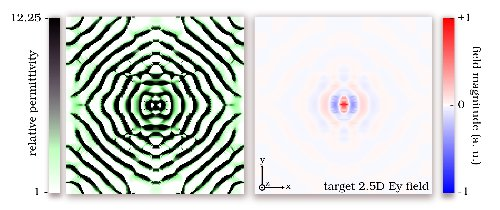
\includegraphics[width=\textwidth]{p2/target}
\caption{The (a) dielectric structure, $\epsilon$, and (b) target field, $E$ ($E_y$ shown only), produced after 75 iterations (10 minutes) on a $160\times 160$ grid. The resulting $\epsilon$ is almost completely binary, and relatively smooth.}\label{target}
\end{figure}
Figs.~\ref{target}a and \ref{target}b are the resulting values of $\epsilon$ and $E$ ($E_y$ shown only), respectively, after 75 iterations of our inverse design method. The entire inverse design process takes only 10 minutes on a standard desktop computer for the $160 \times 160$ grid. 

% The values of the physics residual and the design objective (mode volume) at each iteration are shown in Fig.~\ref{progress}. Most importantly, we see that the physics residual seems to converge linearly, indicating that the algorithm is reasonably efficient. The primary factor in determining this rate of convergence is the exponential decrease in $\eta$ (Eq.~\ref{b1}), since as $\eta$ decreases, increasing emphasis is placed on minimizing the physics residual in the field sub-problem. 
% 
% \begin{figure}[hbt]
% \centering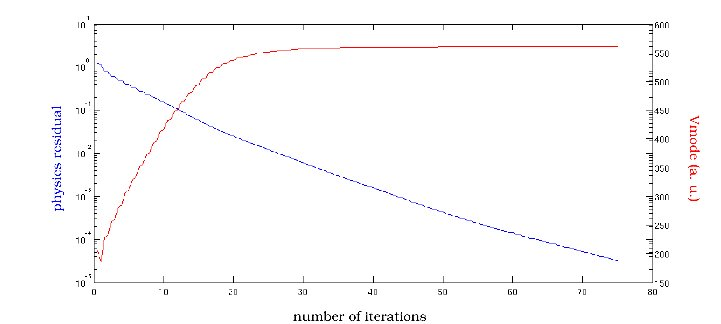
\includegraphics[width=\textwidth]{p2/the_prog}
% \caption{Value of the physics residual (blue) and design objective, or mode volume, (red) at each iteration. The physics residual seems to exhibit linear convergence, while the mode volume quickly saturates after roughly 25 iterations.}\label{progress}
% \end{figure}
% 
To evaluate the accuracy of our 2.5D approximation, we compared the field resulting from the iterations (target field) with the actual field of the resulting structure solved by the 2.5-dimensional approximation (2.5D fiber mode) as well as the field of a full three-dimensional FDTD simulation of the resulting structure (full 3D field), as shown in Figs.~\ref{comp} and \ref{xsec}.

As detailed above, the thickness of the corresponding three-dimensional structure is determined by Eq.~\ref{t}, which yielded a value of $8.16 \Delta x$. However, a small sampling of thicknesses in that vicinity resulted in a more accurate thickness of $8.5\Delta x$, which matched the resonant frequency of the target field and 2.5-dimensional fiber mode.
\begin{figure}[hbt]
\centering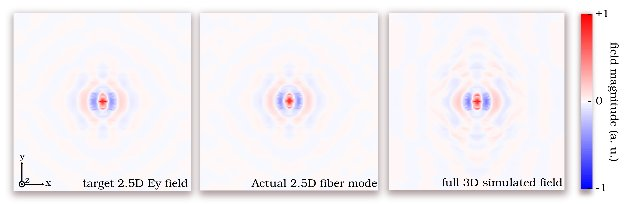
\includegraphics[width=\textwidth]{p2/compare}
\caption{Comparison ($E_y$) of (a) the target field from the inverse design method (from Fig.~\ref{target}), (b) the actual 2.5-dimensional fiber mode, and (c) the field from the full three-dimensional FDTD simulation. The target field matches well with the full three-dimensional field.}\label{comp}
\end{figure}

\begin{figure}[hbt]
\centering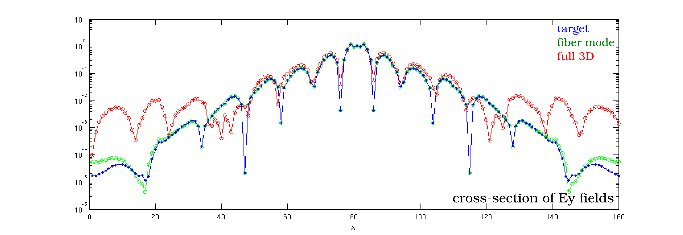
\includegraphics[width=\textwidth]{p2/the_xsec}
\caption{Comparison of the cross sections of the $E_y$ field along the x-axis from the target field (blue), the actual 2.5-dimensional fiber mode (green), and the field from the full three-dimensional FDTD simulation (red). There is some discrepancy between the target field and the full three-dimensional field, but even that is confined to the edges and is only on the order of $\sim 1\%$ of the maximum field amplitude.}\label{xsec}
\end{figure}
Fig.~\ref{comp} plots the $E_y$ component of the target field, 2.5-dimensional fiber mode and the full three-dimensional FDTD field side-by-side. Fig.~\ref{xsec} plots the horizontal cross sections of the magnitudes of the fields on a logarithmic scale. We see that the target field and fiber mode match very well, while there is significantly more discrepancy between the target field and the full three-dimensional field. This is expected with the use of our approximation; however, the error is still relatively small (below 1\% of the maximum field strength) and confined mostly to the edges of the structure.
% 
% \subsection{Performance}
% The fields from the full three-dimensional FDTD simulation were used to evaluate the performance of the device. The resulting mode volume was $0.32 (\frac{\lambda}{n})^3$ and the total quality factor was 7063. The radiative (out-of-plane) quality factor was 8808 and the in-plane quality factor was 35648.
% 
% Fig.~\ref{qcomp} shows the Fourier transforms of the target, fiber and three-dimensional $E_y$ fields taken at the center of the slab. Although there are virtually no field components in the light cone in the case of the target and fiber fields, additional components are present in the full three-dimensional case. This explains why even when leaky radiative components were strictly disallowed in the field optimization sub-problem, the error in the 2.5-dimensional approximation unavoidably introduces some leaky components in the case of the actual three-dimensional structure.
% 
% \begin{figure}[hbt]
% \centering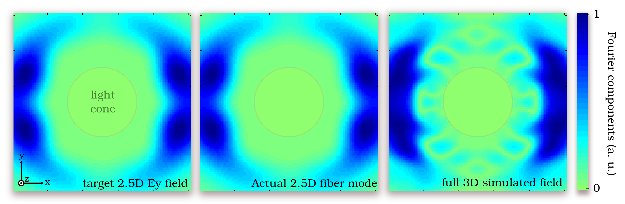
\includegraphics[width=\textwidth]{p2/qcomp}
% \caption{Comparison of the Fourier transforms of the $E_y$ fields of the (a) the target field from the inverse design method, (b) the actual 2.5-dimensional fiber mode, and (c) the field from the full three-dimensional FDTD simulation. The error in our approximation introduces some small additional Fourier components into the light cone.}\label{qcomp}
% \end{figure}
% 
% \section{Conclusion}
% In summary, by using a 2.5-dimension approximation, we demonstrate the inverse design of a three-dimensional nanophotonic resonator. Further development of our method includes applying our inverse method to design three-dimensional devices which support multiple fields at different frequencies. This includes resonant devices such as a multi-wavelength cavity, as well as waveguiding devices such as $N$-port couplers, multiplexers, and grating couplers.\\
% 
